\section{二次函数的形式与图像性质}


\subsection{顶点式}
\label{subsetionL:topponit}

顶点式实际上由一般形式配方而来, 二次函数的顶点式常用于直观表现出二次函数的顶点, 一般式主要体现抛物线与系数的关系

\(y=a(x-h)^2+k\)是顶点式的形式,其中\(k\)和\(h\)的值控制着函数平移的方向和距离,假设有\(y=a(x-h)^2\),若\(h>0\)则函数向左平移,若\(h<0\)则函数向右平移,都是平移\(|h|\)个单位;假设有\(y=ax^2+k\),若\(k>0\)则函数向上平移,若\(k<0\)则函数向下平移,都是平移\(|k|\)个单位.两者一起进行就是顶点式\(y=a(x-h)^2+k\).下面以\(a>0\)时的情况为例说明\(k\)和\(h\)的值如何控制函数:
%%%%%%%%%%%%%%%%%%%%%%%%%%%%%%%%%%%%%%%%%%%%%%%%%%%演示图
\begin{center}
    \begin{tikzpicture}[node distance=7cm]

\centering
\node (start) [] {
\begin{tikzpicture}[
            scale=0.5,
            declare function={
                func(\x) = \x*\x;
            }
        ]
            \draw[->, thick] (-2, 0) -- (2, 0) node[right] {$x$};
            \draw[->, thick] (0, -0.5) -- (0, 3) node[above] {$y$};
        
            \draw[domain=-1.5:1.5, smooth, thick, variable=\x] plot ({\x}, {func(\x)});
            
        \end{tikzpicture}
};
% \node (first) [startstop, above of = start] {从这里开始};
\node (h) [right of=start,yshift=1.5cm] {
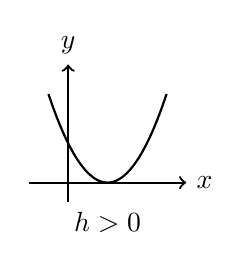
\begin{tikzpicture}[
            scale=0.5,
            declare function={
                func(\x) = (\x-1)*(\x-1);
            }
        ]
            \draw[->, thick] (-1, 0) -- (3, 0) node[right] {$x$};
            \draw[->, thick] (0, -0.5) node[below, xshift=0.5cm] {$h>0$} -- (0, 3) node[above] {$y$};
        
            \draw[domain=-0.5:2.5, smooth, thick, variable=\x] plot ({\x}, {func(\x)});
            
        \end{tikzpicture}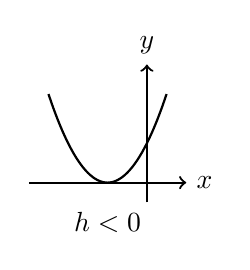
\begin{tikzpicture}[
            scale=0.5,
            declare function={
                func(\x) = (\x+1)*(\x+1);
            }
        ]
            \draw[->, thick] (-3, 0) -- (1, 0) node[right] {$x$};
            \draw[->, thick] (0, -0.5) node[below, xshift=-0.5cm] {$h<0$} -- (0, 3) node[above] {$y$};
        
            \draw[domain=-2.5:0.5, smooth, thick, variable=\x] plot ({\x}, {func(\x)});
            
        \end{tikzpicture}
};
\node (k) [right of=start,yshift=-1.5cm] {
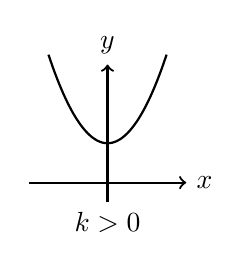
\begin{tikzpicture}[
            scale=0.5,
            declare function={
                func(\x) = \x*\x+1;
            }
        ]
            \draw[->, thick] (-2, 0) -- (2, 0) node[right] {$x$};
            \draw[->, thick] (0, -0.5) node[below] {$k>0$} -- (0, 3) node[above] {$y$};
        
            \draw[domain=-1.5:1.5, smooth, thick, variable=\x] plot ({\x}, {func(\x)});
            
        \end{tikzpicture}
        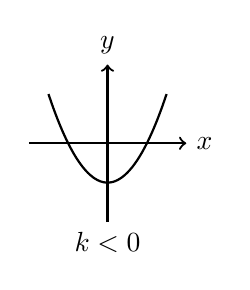
\begin{tikzpicture}[
            scale=0.5,
            declare function={
                func(\x) = \x*\x-1;
            }
        ]
            \draw[->, thick] (-2, 0) -- (2, 0) node[right] {$x$};
            \draw[->, thick] (0, -2) node[below] {$k<0$} -- (0, 2) node[above] {$y$};
        
            \draw[domain=-1.5:1.5, smooth, thick, variable=\x] plot ({\x}, {func(\x)});
            
        \end{tikzpicture}
};

\draw [arrow] (start) -- node[anchor=south, yshift=0.5cm] {$y=(x-h)^2$} (h);
\draw [arrow] (start) -- node[anchor=north, yshift=-0.5cm] {$y=x^2+k$} (k);
\end{tikzpicture}
\end{center}

看图像可以得出当\(a>0\)时,抛物线顶点的纵坐标是函数的最小值;当\(a<0\)时,抛物线顶点的纵坐标是函数的最大值

如果已知抛物线的顶点坐标和抛物线上的另外一个点就能求出抛物线的解析式


\begin{example}
    已知二次函数 \(y = ax^2 + bx + c\),当 \(x = -3\) 时,函数值取得最值 \(4\),当 \(x = 1\) 时,\(y = -8\),则这个二次函数的解析式为\underline{\hspace{5em}}.
    \begin{solution}
        分析:由\(x=-2\),函数值取得最值\(4\)知道抛物线的顶点坐标为\((-3, 4)\),还提供了抛物线上的另外一个点\((1, -8)\),所以确定用顶点式求解析式更快,所以先设解析式\(y=a(x-h)^2+k\),再代入\(h,k\)的值,然后只剩参数\(a\),代入另外一个点\((1, -8)\)即可求得解析式.设解析式为$y = a(x - h)^2 + k$再代入 \(h, k\) 的值,只剩参数 \(a\),代入另一点即可求出.

        
        \[
\begin{alignedat}{3}
&\text{设解析式为 } y = a(x - h)^2 + k, &\quad
&\because x = -3 \text{ 时函数值取得最值 } 4, &\quad
&\therefore \text{顶点为 } (-3,4), \\[2pt]
&\therefore y = a(x+3)^2 + 4, &
&\because (1,-8) \text{ 在抛物线上}, &
&-8 = a(1+3)^2 + 4, \\[2pt]
&-8 = 16a + 4, &
&16a = -12, &
&a = -\dfrac{3}{4}, \\[2pt]
&\therefore y = -\frac{3}{4}(x+3)^2 + 4, &
&= -\frac{3}{4}(x^2 + 6x + 9) + 4, &
&= -\frac{3}{4}x^2 - \frac{9}{2}x - \frac{27}{4} + \frac{16}{4}, \\[2pt]
& & & & &y = -\frac{3}{4}x^2 - \frac{9}{2}x - \frac{11}{4}
\end{alignedat}
\]

        
        
    \end{solution}
\end{example}


%顶点式的关键是顶点坐标为(h,k)

\subsection{一般式}
二次函数一般式:\(y=ax^2+bx+c\).

顶点式实际上由一般形式配方而来, 二次函数的顶点式常用于直观表现出二次函数的顶点, 一般式主要体现抛物线与系数的关系:


二次函数的一般式为:
\[
y = ax^2 + bx + c\quad (a \neq 0)
\]
其中,$a$、$b$、$c$ 为常数,$a$ 决定开口方向与宽窄,$b$ 影响对称轴位置,$c$ 为纵截距(截距指函数与y轴的交点的纵坐标).

二次函数的一般式可以通过配方化为顶点式 $y = a(x - h)^2 + k$,其中 $(h,k)$ 为顶点坐标.

从一般式出发:
\[
y = ax^2 + bx + c
\]
提取 $a$:
\[
y = a\left(x^2 + \frac{b}{a}x\right) + c
\]
在括号内配方:
\[
y = a\left[x^2 + \frac{b}{a}x + \left(\frac{b}{2a}\right)^2 - \left(\frac{b}{2a}\right)^2 \right] + c
\]
整理:
\[
y = a\left(x + \frac{b}{2a}\right)^2 - \frac{b^2}{4a} + c
\]
由此得到顶点式:
\[
y = a\left(x + \frac{b}{2a}\right)^2 + \left(c - \frac{b^2}{4a}\right)  \quad\Rightarrow\quad y = a\left(x + \frac{b}{2a}\right)^2 + \frac{4ac-b^2}{4a}
\]
可以推出顶点坐标为:
\[
h = -\frac{b}{2a}, \quad k = \dfrac{4ac-b^2}{4a}
\]

如果已知一般式要求顶点不想配方,就可以套用$h = -\dfrac{b}{2a}, \quad k = \dfrac{4ac-b^2}{4a}$,一般式也可以反映对称轴即顶点的横座标:\(x=-\dfrac{b}{2a}\)
总结一般式的性质如下:
\begin{enumerate}
    \item 对称轴:$x = -\dfrac{b}{2a}$
    \item 顶点:$\left(-\dfrac{b}{2a},\ \dfrac{4ac-b^2}{4a}\right)$
    \item 开口方向:$a > 0$ 向上开口;$a < 0$ 向下开口
\end{enumerate}

%%%%%%%%%%%%%%%%%%%%%%%%%%%%%%%%%%%%%%%%%%%%%%%%%%%%%%%%%%%%%%%%%%%%%%%%%%%%%%%%%此处未遍例题

“一般式主要体现抛物线与系数的关系”,你是否联想到了韦达定理(根与系数的关系)?


\subsection{交点式(两根式/因式分解式)}
\textbf{交点式:\(y=a(x-x_1)(x-x_2) \quad (\Delta>0)\)}

交点式常用于直观表现直观表现二次函数与\(x\)轴的交点坐标.

\textbf{推导:}二次函数的一般式为:
\[
y = ax^2 + bx + c, \quad a \neq 0
\]
如果它在 $x$ 轴上有两个实数交点 $x_1$ 和 $x_2$(即二次方程 $ax^2 + bx + c = 0$ 有实根),
那么函数可以写成交点式(因式分解式):
\[
y = a(x - x_1)(x - x_2)
\]


设二次方程 $ax^2 + bx + c = 0$ 的两个实根为 $x_1$ 和 $x_2$,由韦达定理:
\[
x_1 + x_2 = -\frac{b}{a}, \quad x_1 x_2 = \frac{c}{a}
\]
则:
\[
ax^2 + bx + c 
= ax^2-\dfrac{b}{a}x+\dfrac{c}{a}
= \underbrace{a\left[x^2 - (x_1 + x_2)x + x_1 x_2\right]}_{\text{提取公因数\(a\)}}
\]
代入根与系数关系:
\[
= a\left[x^2 - \left(-\frac{b}{a}\right)x + \frac{c}{a}\right]
= a\left(x - x_1\right)\left(x - x_2\right)
\]
所以二次函数的交点式为:
\[
y = a(x - x_1)(x - x_2)
\]

交点式便于直接观察函数与\(x\)轴的交点,由于教材没有介绍交点式,所以不要在书写题目过程的时候使用交点式,可以在选填或检验的时候使用交点式快速得到答案.

使用交点式的前提是$\Delta > 0$,特别的,\textbf{当\(\Delta=0\)时,交点式退化为$y = a(x - p)^2$},如果$\Delta < 0$,由于二次函数与\(x\)轴无交点,所以不能写成交点式,需要根据情况写成顶点式或一般式.总结交点式的性质如下:

\begin{enumerate}
    \item 交点式中的 $x_1$、$x_2$ 为函数图像与 $x$ 轴的交点横坐标.
    \item 当 $a > 0$ 时,抛物线开口向上;当 $a < 0$ 时,抛物线开口向下.(与顶点式和交点式相同)
    \item 交点式可直观反映零点位置与图像对称性.(零点指二次函数\(y=ax^2+bx+c\)的\(y=0\)时\(x\)的值,即方程\(ax^2+bx+c=0\)的解)
\end{enumerate}

%%%%%%%%%%%%%%%%%%%%%%%%%%%%%%%%%%%%%%%%%%%%%%%%%%%%%%%%未编写例题